\documentclass{article}
\usepackage{pgfplots}
\title{KEEL: ROC output}
\begin{document}
\maketitle
\hfill \break
File: TEST
\hfill \break
\hfill \break
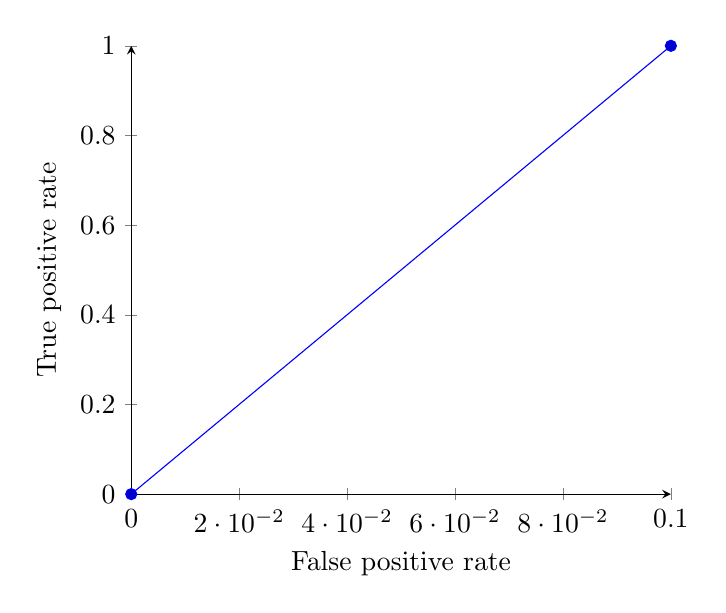
\begin{tikzpicture}
\begin{axis} [xlabel=False positive rate,
ylabel=True positive rate,axis x line=bottom,
axis y line=left]
\addplot coordinates { (0,0)(0.1,1.0) };\end{axis}
\end{tikzpicture}\hfill \break
 AUC:0.05
\hfill \break
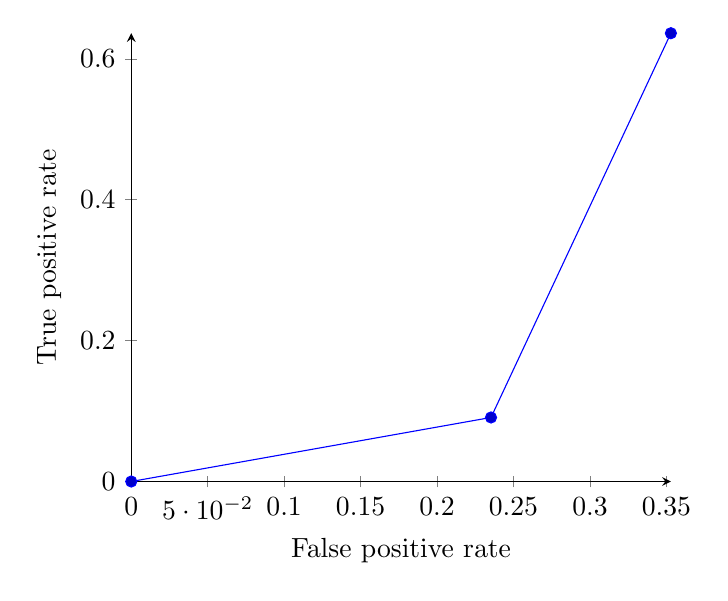
\begin{tikzpicture}
\begin{axis} [xlabel=False positive rate,
ylabel=True positive rate,axis x line=bottom,
axis y line=left]
\addplot coordinates { (0,0)(0.23529411764705882,0.09090909090909091)(0.35294117647058826,0.6363636363636365) };\end{axis}
\end{tikzpicture}\hfill \break
 AUC:0.05347593582887702
\hfill \break
\begin{tikzpicture}
\begin{axis} [xlabel=False positive rate,
ylabel=True positive rate,axis x line=bottom,
axis y line=left]
\addplot coordinates { (0,0)(0.39285714285714274,0.14285714285714285) };\end{axis}
\end{tikzpicture}\hfill \break
 AUC:0.028061224489795908
\hfill \break
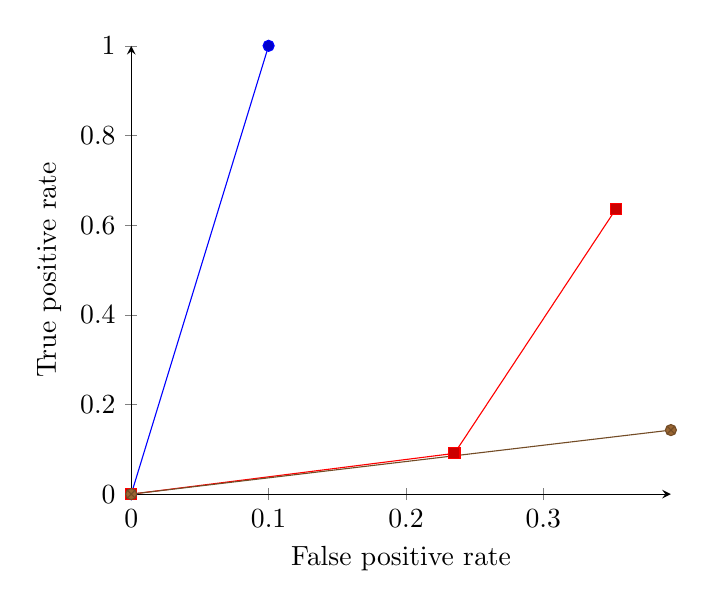
\begin{tikzpicture}
\begin{axis} [xlabel=False positive rate,
ylabel=True positive rate,axis x line=bottom,
axis y line=left]
\addplot coordinates { (0,0)(0.1,1.0) };
\addplot coordinates { (0,0)(0.23529411764705882,0.09090909090909091)(0.35294117647058826,0.6363636363636365) };
\addplot coordinates { (0,0)(0.39285714285714274,0.14285714285714285) };
\end{axis}
\end{tikzpicture}\hfill \break
File: TRAINING
\hfill \break
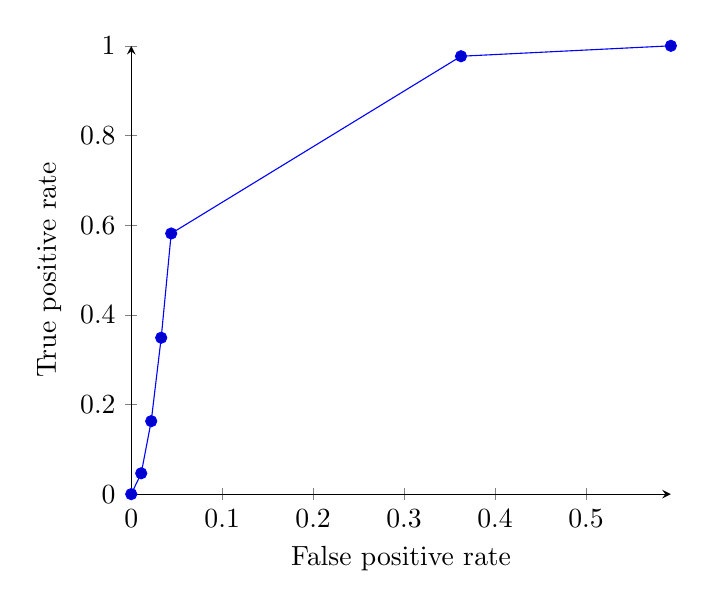
\begin{tikzpicture}
\begin{axis} [xlabel=False positive rate,
ylabel=True positive rate,axis x line=bottom,
axis y line=left]
\addplot coordinates { (0,0)(0.01098901098901099,0.046511627906976744)(0.02197802197802198,0.16279069767441862)(0.03296703296703297,0.3488372093023255)(0.04395604395604396,0.5813953488372092)(0.3626373626373627,0.9767441860465123)(0.5934065934065933,1.0000000000000007) };\end{axis}
\end{tikzpicture}\hfill \break
 AUC:0.48556095067722993
\hfill \break
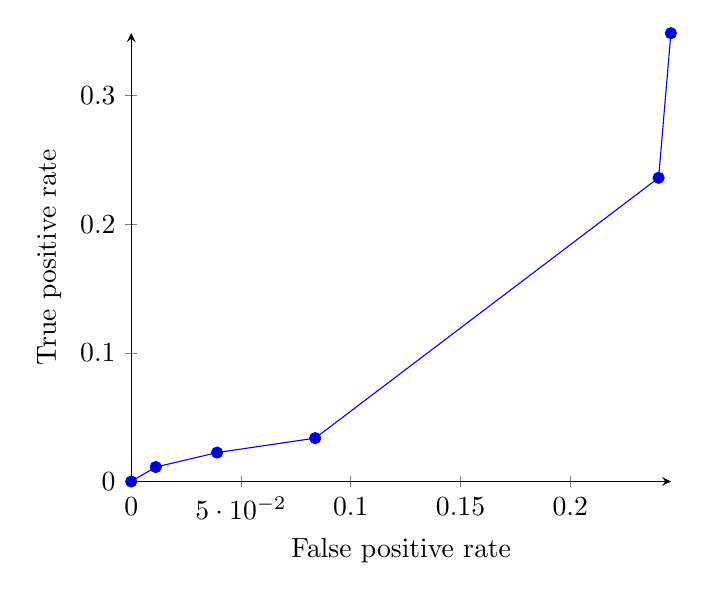
\begin{tikzpicture}
\begin{axis} [xlabel=False positive rate,
ylabel=True positive rate,axis x line=bottom,
axis y line=left]
\addplot coordinates { (0,0)(0.0111731843575419,0.011235955056179775)(0.03910614525139665,0.02247191011235955)(0.08379888268156423,0.033707865168539325)(0.24022346368715067,0.23595505617977527)(0.2458100558659216,0.3483146067415732) };\end{axis}
\end{tikzpicture}\hfill \break
 AUC:0.05090703659531726
\hfill \break
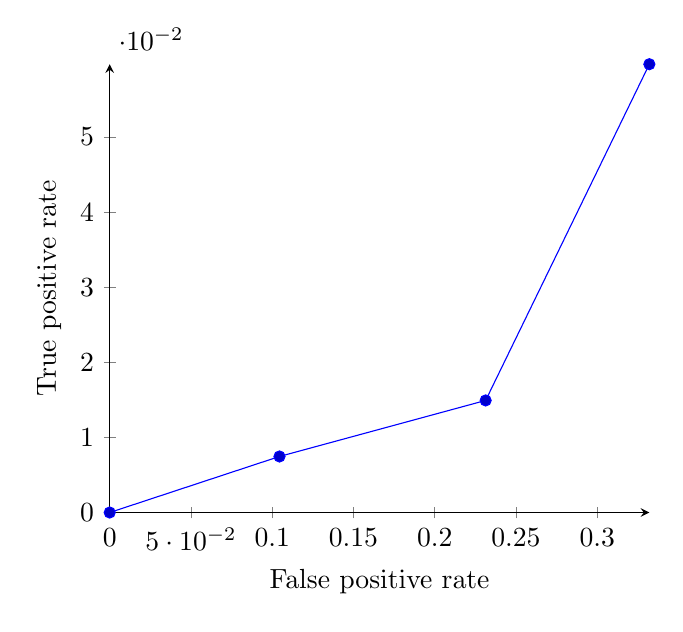
\begin{tikzpicture}
\begin{axis} [xlabel=False positive rate,
ylabel=True positive rate,axis x line=bottom,
axis y line=left]
\addplot coordinates { (0,0)(0.10447761194029845,0.007462686567164179)(0.23134328358208978,0.014925373134328358)(0.3320895522388065,0.05970149253731343) };\end{axis}
\end{tikzpicture}\hfill \break
 AUC:0.008952439296057052
\hfill \break
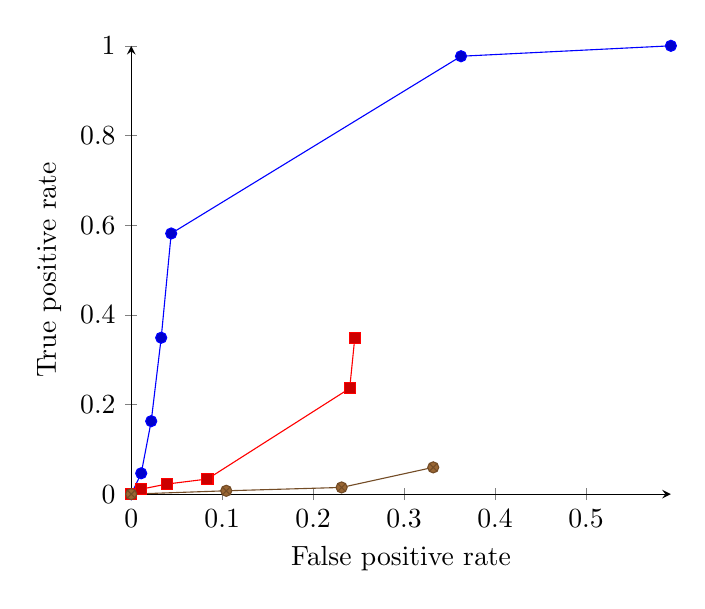
\begin{tikzpicture}
\begin{axis} [xlabel=False positive rate,
ylabel=True positive rate,axis x line=bottom,
axis y line=left]
\addplot coordinates { (0,0)(0.01098901098901099,0.046511627906976744)(0.02197802197802198,0.16279069767441862)(0.03296703296703297,0.3488372093023255)(0.04395604395604396,0.5813953488372092)(0.3626373626373627,0.9767441860465123)(0.5934065934065933,1.0000000000000007) };
\addplot coordinates { (0,0)(0.0111731843575419,0.011235955056179775)(0.03910614525139665,0.02247191011235955)(0.08379888268156423,0.033707865168539325)(0.24022346368715067,0.23595505617977527)(0.2458100558659216,0.3483146067415732) };
\addplot coordinates { (0,0)(0.10447761194029845,0.007462686567164179)(0.23134328358208978,0.014925373134328358)(0.3320895522388065,0.05970149253731343) };
\end{axis}
\end{tikzpicture}\end{document}